\chapter{Implementation} \label{implementation}
This chapter will elaborate on the test data used as well as the process that was followed to achieve the results in Chapter \ref{results}.
\section{Existing data}
The data used was acquired by \cite{Westhuyzen:2020} for an article assessing the charring rate of both SA-Pine and Eucalyptus.
	For the purpose of this project, only the data obtained from the SA-Pine test was considered and analysed. 
	\subsection{Summary of test}
	The test was conducted on a sample panel of $100$ mm by $0.9$ m $\times 0.9$ m cross-laminated SA-pine.
	This sample was then divided into nine cubes of $100$ mm $\times 100$ mm $\times 100$ mm.
	%The sample was a 100 mm by 0.9m x 0.9m panel of cross-laminated SA-pine, this sample was then divided into nine cubes of 100 mm x 100 mm x 100 mm.
	Each cube was fitted with seven Type K-thermocouples placed at consecutive $16.5$ mm drilled holes, as can be seen in Figure \ref{TC_layout}. 
	The test panel was tested in a furnace and was exposed to the standard ISO 834 Fire curve \ref{firecurve_fig} on one side and room temperature on the other. 
	The panel was exposed to the fire curve for $50$ minutes, at which stage near complete de-lamination was observed and the test ended.
	\begin{figure}[H]
	\centering
	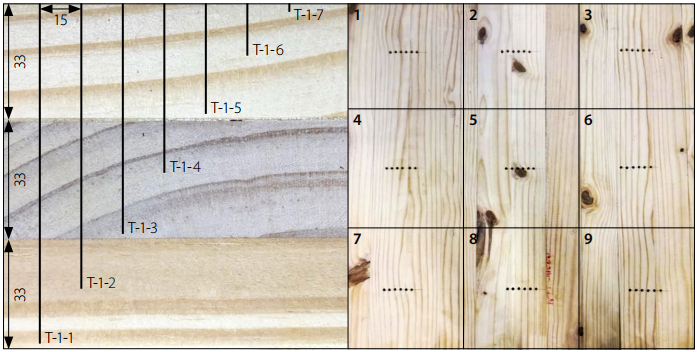
\includegraphics[width=0.75\linewidth]{figures/TC_layout.png}
	\caption{Thermocouple layout in test conducted by \cite{Westhuyzen:2020} cross-section (left) and overall layout (right)}
	\label{TC_layout}
	\end{figure}
	
	\begin{figure}[H]
	\centering 
	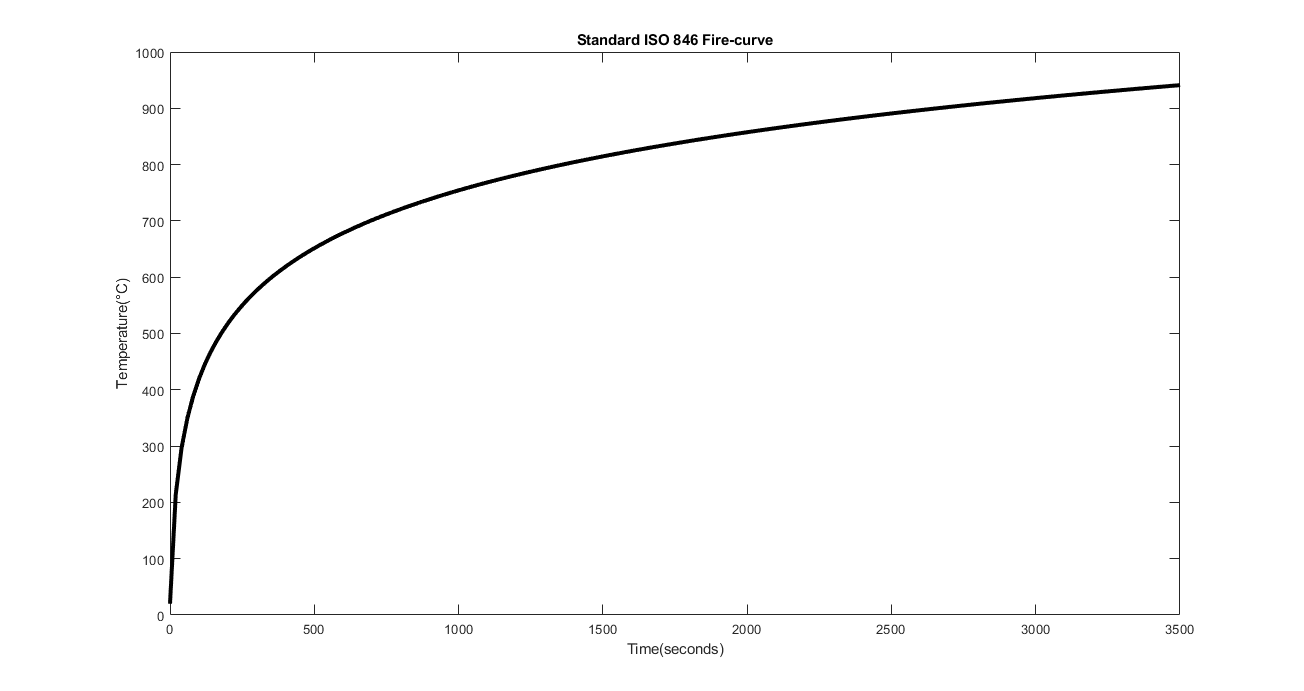
\includegraphics[width=\linewidth]{figures/firecurve.png}
	\caption{Standard ISO fire curve TODO}
	\label{firecurve_fig}
	\end{figure}
	In Figure \ref{measured_fig} 
	\begin{figure}[H]
	\label{measured_fig}
	\centering
	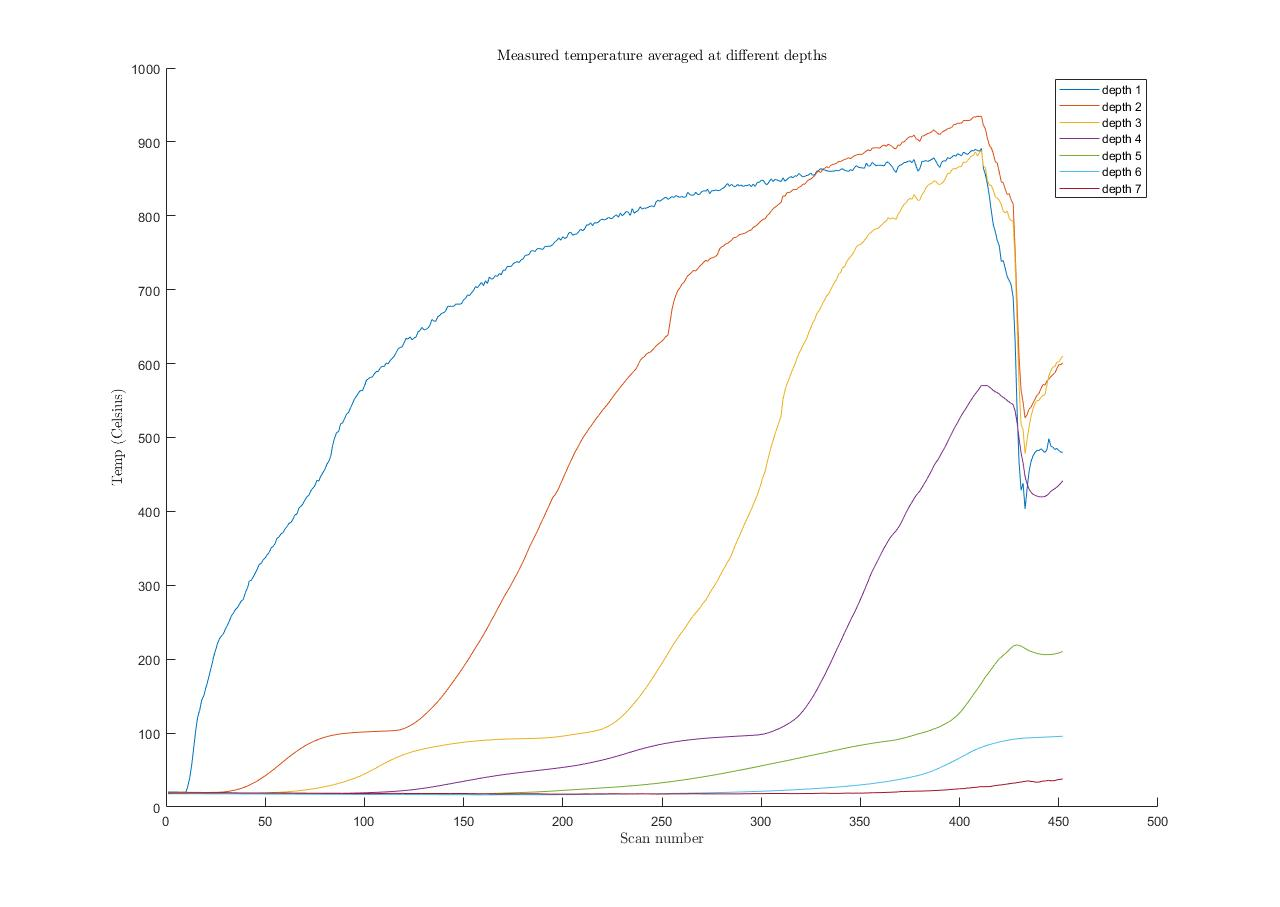
\includegraphics[width=5.5in,]{figures/measured_data.jpg}
\end{figure}

	\subsection{Potential inaccuracies}
	As with most tests, everything is not always perfect. 
	The potential inaccuracies are discussed below. 	
	In the data, it was observed that two of the thermocouples broke during testing; this resulted in temperature with a magnitude of $10^{13}$. 
	Such a temperature is impossible, as the highest ever recorded temperature reached was $4\times 10^{12}$ and that only occurred in a atomic explosion. %(https://www.insidescience.org/news/hottest-temperature-universe-measured)% 
	This malfunction required that two of the depth measurements were no longer the average between nine samples but instead the average between eight.
	Another inaccuracy that could potentially influence the accuracy of the final result is the accuracy of the depth of the holes in which the thermocouples were placed. 
	%As this was done by hand in the laboratory.
	
	There is also debate about the significance of the contribution of the timber burning to the temperature inside the furnace. 
	For the purposes of this project, it will be assumed that the timber burning does not contribute to the temperature inside the furnace.
	
\section{Finite Element Modelling}\label{femexpl}
A one-dimensional finite element model that simulates what we expect to obtain from the fire tests based on the simplified $\kappa$-values provided in EN 1995:1-2-2004 is modified into a function.
This function should provide the temperature of the modelled element based on a specified location and thermal conductivity.
The derivation and adaptation of the model are expanded on below.
	\subsection{Derivation}%"CREATION?"
	%The assumption that the panel is constantly at room temperature on the outside is also inaccurate as there is heat radiating from the panel that increases the temperature surrounding the panel.
	
	Assumptions were made to simplify the model, they were as follows
	\begin{enumerate}
\item{The air on the side of fire follows the temperature of the fire curve.}
\item{The air on the cold side remains at 20$^{^\circ}$C.}
	\end{enumerate}
	\subsubsection{Stationary heat conduction}
	\begin{figure}[H]
	\label{femfig}
	\centering
	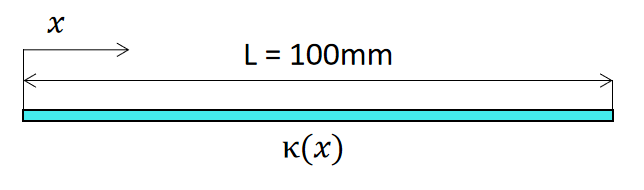
\includegraphics[width = 0.75\linewidth]{figures/fem_sketch.png}
	\caption{Visualisation of element that is modelled in one-dimension}
	\end{figure}
	The derivation started as a one-dimensional stationary heat conduction problem with the below equations as a starting point.
	\begin{equation}
	\label{heateq1}
	q_{,x}-f = 0  \text{  ...(1)} \quad\quad\quad\quad q = -\kappa u_{,x} \text{  ...(2)} 
	\end{equation}
	Integrating Equation \ref{heateq1} (1) over the length of the element(shown in Figure \ref{femfig}) and introducing a weighting function $w(x)$ we obtain \ref{heateq2}. 
	Since the derivative of $w(0)$ is known and $q_{,x}$ is unknown. 
	The first term in \ref{heateq2} is integrated by parts. 
	After the integration by parts and substituting $q$ with \ref{heateq1} (2), Equation \ref{heateq3} is created.
	\begin{equation}
	\label{heateq2}
	\int_{x=0}^L wq_{,x}dx - \int_{x=0}^L wfdx = 0
	\end{equation}
	\begin{equation}
	\label{heateq3}
	\int_{x=0}^L wku_{,x}dx + \int_{x=0}^L wfdx - \left.wq\right|_0^L = 0
	\end{equation}
	In Equation \ref{heateq3} the $u$ and $w$ need to be defined.
	Assuming $u \approx u^h$ and $w \approx w^h$ and using the basis function ($N^A$), Equation \ref{basisfunc_eq} is obtained.
	\begin{equation}
	\label{basisfunc_eq}
	\begin{aligned}
	u_e^h = \sum_{B} N^B d^B  \quad &;\quad w_e^h = \sum_{A} N^A c^A\\
	u_{e,x}^h = \sum_{B} N_{,x}^B d^B \quad &;\quad w_{e,x}^h=\sum_A N_{,x}^A c^A\\
	\end{aligned}
	\end{equation}		
	Substituting the $u$ and $w$ functions back, we obtain the Galerkin weak form shown in Equation \ref{heateq4}.
	In Equation\ref{heateq4} the $A_N$ referes to the nodes that have Newmann boundaries(TODO explained in \ref{femsec}). 
	The variables $c^A$ and $d^B$ are independant of x and can therefore be taken out of the integral. 
	The sum over A and B are also taken out of the integral.
	When the summing is applied a matrix of all the possible combinations between A and B can be used to replace the sum. The resulting matrices are shown in Equation \ref{heateq5}. 
	When written in matrix form the summing is implied, if matrix form is it written then the expression referrers to the terms that will still be summed.

	\begin{equation}
	\label{heateq4}
	\begin{aligned}
	\sum_e \int_{\Omega_e} w_{e,x}^h k  u_{e,x}^h dx &+ \sum_e \int_{\Omega_e} w_e^h f dx - w(L)q_L + w(0)q_0 &= 0\\
	\int_{\Omega_e} \sum_A \sum_B N_{,x}^A c^A k N_{,x}^B d^B dx  &+ \int_{\Omega_e} \sum_{A} N^A c^A f dx - \sum_{A\in A_N} c^A q^A &= 0\\
	\end{aligned}
	\end{equation}
	\begin{equation}
	\label{heateq5}
	\vec{c}_e^T \vec{K}_e^{AB} \vec{d}_e + \vec{c}_e^T \vec{F}_e^f -\vec{c}_e^T \vec{F}_e^q
	\end{equation}
	where
	\begin{equation*}
	\begin{aligned}
	K_e^{AB} &= \int_{\Omega_e}N_{,x}^AN_{,x}^B k dx\\
	F_e^{Af} &= \int_{\Omega_e}N_{,x}^A f dx\\
	F_e^{Aq} &= \begin{cases} q(x_N) &\text{ for } x \in \Gamma_N\\0 &\text{ for other }\\
	\end{cases}
	\end{aligned}
	\end{equation*}
	
	\subsubsection{Boundaries}
	\begin{figure}[H]\label{airelmfig}
	\centering
	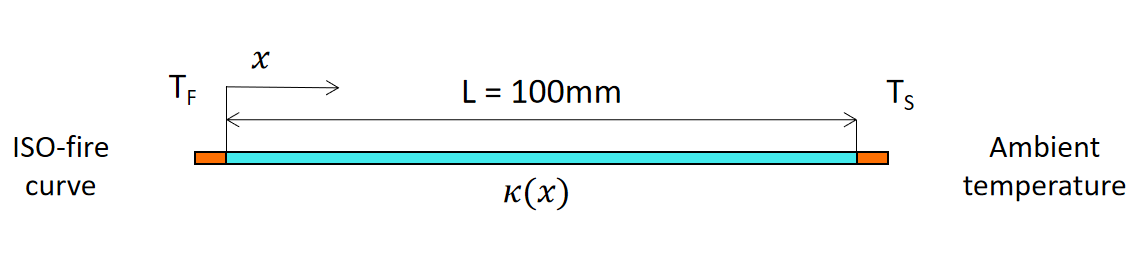
\includegraphics[width = 0.75\linewidth]{figures/fem_fire_sketch.png}
	\caption{Visualisation of one-dimensional element with air elements and external conditions added}
	\end{figure}
	
	One of the additional difficulties in modelling is that the known boundary temperatures are measured in the air of the furnace and assumed for the air outside the furnace.
	Initially a long element of air was modelled.
	This element is then overlaid with the timber element to effectively add an air element it each end of the timber element as depicted in \ref{airelmfig}
	In the air elements, both heat convection and heat radiation need to be taken into account.
	The equations for heat convection and radiation can be seen in Equation \ref{heatconeq} and \ref{radeq}.
	
	\begin{equation} \label{heatconeq}       
	       \begin{aligned}
	       q_{\text{adv}}= \nu &\rho c_p \Delta T \quad = \quad h \Delta T\\	      
	       \nu =& \text{velocity m/s}\\
	       \rho =& \text{density of air}\\
	       c_{\rho} =& \text{heat capacity of air}\\
          \end{aligned}
	\end{equation}
	       
	\begin{equation} \label{radeq}
	       \begin{aligned}
	       q_{\text{rad}} = \varepsilon&\sigma \phi \left(T_f^4 - T_S^4\right)\\
	       \varepsilon =& \text{emissivity}\\
	       \sigma =& \text{Stefan-Boltzmann} \\&5.670 e^-8 [W/(m^2K^4)]\\
	       \phi =& \text{view factor};1 \quad \text{here}\\
	       \end{aligned}
	\end{equation}
	Given that $T_S$ and $T_F$ are known a new equivalent heat flux value can be calculated as in Equation \ref{femboundeq1}.
	\begin{equation} \label{femboundeq1}
	q_{\text{con}}^{\text{equiv}} = \kappa^{\text{equiv}} \frac{\Delta T}{\Delta L} = q_{\text{rad}} + q_{\text{adv}}\\
	\end{equation}
	Due to the clear relationship between heat flux and thermal diffusivity the equivalent diffusivity($\kappa^{\text{equiv}}$) can be calculated as shown below in Equation \ref{femboundeq2}. 
	\begin{equation}\label{femboundeq2}
	\begin{aligned}
	\kappa^{\text{equiv}} &= \frac{\left[q_{\text{rad}} + q_{\text{adv}} \right]}{\Delta T}\\
	&\quad\\
	&= \frac{\epsilon \sigma \phi \Delta \left(T^4\right)}{\Delta T / \Delta L } + h \Delta L\\
	&\quad\\
	&= \frac{\epsilon \sigma \Delta \left(T^4\right)}{\Delta T   } + h\\
	\end{aligned}
	\end{equation}
	
	\subsubsection{One-dimensional diffusion}
The concept of diffusion is thoroughly explained in \ref{femsec}(TODO) below the mathematical application is explained and steps that were taken to obtain the final model is shown.
	\begin{equation}\label{femdiffeq1}
	q_{,x} - f = \frac{\partial Q}{\partial t} = c_{\rho}\frac{\partial u}{\partial t}\quad\text{  ...(1)} \quad\quad\quad q = -\kappa \frac{\partial u}{\partial x}\quad\text{  ...(2)}
\end{equation}
Substituting Equation \ref{femdiffeq1}(2) into \ref{femdiffeq1} and taking the derivative as indicated ($q_{,x}$) gives Equation \ref{femdiffeq2}. 
As previously disccussed heat conduction ($\alpha$) is heat diffusion ($\kappa$)  divided by specific heat ($c_p$).


\begin{equation}\label{femdiffeq2}
\begin{aligned}
\therefore -\kappa \frac{\partial^2 u}{\partial x^2} - f &= c_{\rho}\frac{\partial u}{\partial t} \rightarrow f=0:\\
\frac{\partial^2 u}{\partial x^2} &= - \frac{c_{\rho}}{\kappa} \frac{\partial u}{\partial t} \quad \\
&\text{ or } \\
\frac{\partial u}{\partial t} &= -\alpha \frac{\partial^2 u}{\partial x^2}
\end{aligned}
\end{equation}


Let $c_p = \lambda$ 

\begin{equation}\label{femdiffeq3}
\therefore -\kappa u_{,xx} - \lambda u_{,t} = f
\end{equation}


Then:

\begin{equation}\label{femdiffeq4}
\int_0^L w q_{,x} \text{d}x - \int_0^L w \lambda u_{,t} \text{d}x - \int_0^L w f \text{d}x = 0
\end{equation}


Similar to what was done in \ref{basisfunc_eq} a special approximation is made to obtain Equation \ref{femdiffeq5}.

\begin{equation}\label{femdiffeq5}
u \approx u^h \rightarrow u_e^h = \sum_{A}N^A d^A \quad;\quad w_e^h = \sum_{A}N^A L^A
\end{equation}


\begin{equation}\label{femdiffeq6}
\rightarrow \sum_e \int_{\Omega^e} w_{e,x}^h \kappa u_{e,x}^h \text{d}x_e + \sum_e \int_{\Omega^e} w_e^h \lambda u_{e,t}^h \text{d}x_e + \sum_e \int_{\Omega^e} w_e^h f \text{d}x_e - \sum_{e \in \epsilon_A} w q_N = 0
\end{equation}

\begin{equation*}
*_1: \int_{\Omega^e} \sum_A \sum_B N_{,x}^A c^A \kappa N_{,x}^B d^B \text{d}x = \sum_A\sum_B \left[ \int N_{,x}^A N_{,x}^B \kappa \text{d}x  \right]d^B = \vec{c}_e^T \vec{\kappa}_e \vec{d}_e
\end{equation*}


\begin{equation*}
*_2: \int_{\Omega_e} \sum_A \sum_B N^A c^A \lambda N^B \dot{d}^B \text{d}x = \sum\sum c^A \left[ \int N^A N^B \lambda \text{d}x \right] d^B = \vec{c}_e^T \vec{M}_e \vec{\dot{d}}_e
\end{equation*}


\begin{equation*}
*_3: \int_{\Omega^e} \sum_A N^A c^A f \text{d}x = \sum c \int_B^A N f \text{d}x = \vec{c}_e^T \vec{F}_e^B
\end{equation*}


\begin{equation*}
*_4: \sum_{A \in \mathcal{A}} \kappa^A q_N^A = \vec{c}_e^T \vec{F}_e^q
\end{equation*}


From all the above equations the below matrix formulation could be assembled:
%considere renamin to somehing with assembled or matrix in the name
\begin{equation}\label{femdiffeq7}
\vec{c}^T \vec{\kappa} \vec{d} + \vec{c}^T \vec{M} \vec{\dot{d}} = \vec{c}^T \vec{F}
\end{equation}


Solving:(TODO: date 15/10 last)

\begin{equation}
(1) \text{ Set } \vec{d}_0 = |---|---|---| \\
\&\ \vec{v}_0 = \vec{0} \\
\text{Also set } \alpha \text{ (mixing constant?)} ; \Delta t
\end{equation}


\begin{equation}
(2) \text{ Time integration [v-form;Hughes Ch8]} \\
\vec{d}_{n+1} = \vec{d}_n + (1-\alpha) \Delta \vec{v}_n + \alpha \Delta t \vec{v}_{n+1}
\end{equation}


\begin{equation}
(\vec{M} + \alpha\Delta t \vec{\kappa})\vec{v}_{n+1} = \vec{F}_{n+1} - \vec{\kappa} \tilde{\vec{d}}_{n+1}
\end{equation}


if $\vec{M}$ and $\vec{\kappa}$ independent of time and temperature, sufficient to say:

\begin{equation}
\vec{v}_{n+1} = (\vec{M}+\alpha\Delta t \vec{\kappa})^{-1} (\vec{F}_{n+1} - \vec{\kappa} \vec{\tilde{d}}_{n+1})
\end{equation}

%Page 5 
If $\kappa$ and $\lambda$ is independent of position:
\begin{equation}
\begin{aligned}
	\kappa_e^{AB} &= \int_0^\ell N_{,x}^A N_{,x}^B \kappa \text{d}x \\
&= \kappa \int_0^\ell N_{,x}^A N_{,x}^B \text{d}x \\
&= \kappa \int_{-1}^{+1} N_{,\xi}^A N_{,\xi}^B \xi_{,x}^2 \left|J\right|  d\xi \\
&=\kappa \frac{2}{\ell} \int_{-1}^{+1} N_{,\xi}^A N_{,\xi}^B \text{d}\xi\\
&= \pm \frac{\kappa}{\ell} = \begin{cases}
+\frac{1}{2} & \text{if } A = B \\
-\frac{1}{2} & \text{if } A \ne B
\end{cases}
\end{aligned}
\end{equation}

\begin{equation}
\therefore \vec{\kappa}_e = \frac{\kappa}{\ell} \begin{bmatrix} +1 & -1 \\ -1 & +1 \end{bmatrix}
\end{equation}	

\begin{equation}
M_e^{AB} = \int_0^\ell N^A N^B \lambda \text{d}x = \lambda \int_0^\ell N^A N^B \text{d}x = \frac{\lambda \ell}{2} \int_{-1}^{+1} N^A N^B \text{d}x
\end{equation}
\begin{equation}
N^1 N^1 = \frac{1}{4}(1-\xi)^2 ; N^2 N^2 = \frac{1}{4}(1+\xi)^2 ; N^1 N^2 = \frac{1}{4}(1-\xi^2)
\end{equation}

\begin{equation}
N^1 = \frac{1-\xi}{2} ; N^2 = \frac{1+\xi}{2}
\end{equation}

Then
	\begin{equation}
	\begin{aligned}
	\int N^1 N^1 &= \frac{1}{4} \left[ \xi + \frac{1}{3}\xi^3 \right]_{-1}^{+1} = \frac{2}{3} \\
	\int N^2 N^2 &= \frac{1}{4} \left[ \xi + \frac{1}{3}\xi^3 \right]_{-1}^{+1} = \frac{2}{3} \\
	\int N^1 N^2 &= \frac{1}{4} \left[ \xi - \frac{1}{3}\xi^3 \right]_{-1}^{+1} = \frac{1}{3} \\
	\end{aligned}
	\end{equation}	
	
	\begin{equation}
	\therefore \vec{M}_e = \frac{\lambda \ell}{6} \begin{bmatrix} 2 & 1 \\ 1 & 2 \end{bmatrix}
	\end{equation}
	
	\begin{equation}
	\vec{F}_e^{fA} = \int_0^\ell N f \text{d}x = f \frac{\ell}{2} \int_{-1}^{+1} N \text{d}x = f\frac{\ell}{2} \\
\therefore \vec{F}_e^f = \frac{f\ell}{2} \begin{Bmatrix} 1\\1 \end{Bmatrix}
	\end{equation}
	\subsection{Existing Model}
	For this project an existing finite element model of heat diffusion by Prof. N de Koker was modified for usage in the Bayes' theorem~\ref{bayes_eq}. 
	This model is used to determine the likelihood function. 
	The current model uses the standard Euro code $\kappa$-values as well as the specific heat specified in the \citep{Euro:2004}. 
	
	The model discretises the wooden element into 32 different elements. For finite element analysis, there are always more elements used to generate the model than usually evaluated. This is done to improve the accuracy of said model.
	The model is a one dimensional finite element model that takes time differentiation into account.
	
\begin{figure}[H]
	\label{og_modeldata}
	\centering
	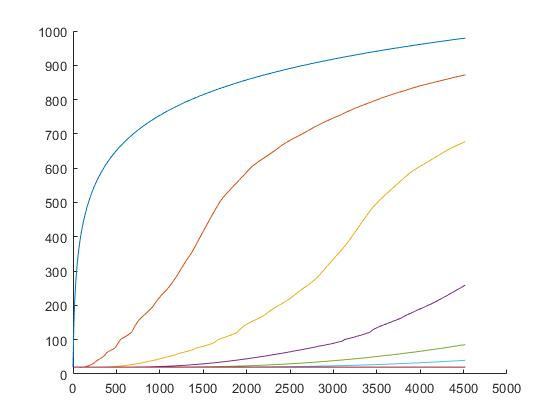
\includegraphics[width=\linewidth,]{figures/originalmugraph.jpg}
	\caption{Output of finite element model using $\kappa$-values as indicated in EN 1995:1-2-2004}
\end{figure}	

	\subsection{Adapted Model}	
	The model was changed into a function that takes $\kappa$-values and provides a new temperature distribution over the elements for the different $\kappa$-values. 
	This function is used in the posterior calculation to determine the likelihood function.
	

\section{Inversion method}
%here we will discuss everything that we did
The basis of the stochastic analysis is the adapted Bayesian equation \ref{modbayes} below. 
TODO: further interpret

\begin{equation}
\label{modbayes}
\pi^* (x|T) = \exp\left(-\frac{(\mu - x)^2}{2\sigma_{\mu}^2}\right) \cdot \exp\left(-\frac{\left(T-M(x)\right)^2}{2\sigma_{\text{temp}}^2}\right)
\end{equation}

	\subsection{Prior probability}
	
	\begin{equation}
	\label{prior}
	\pi(x) = \exp\left(-\frac{(\mu - x)^2}{2\sigma_{\mu}^2}\right)
	\end{equation}

	The prior probability function (Equation \ref{prior} ) is based on the $\kappa$-values assumed prior to any simulation or analysis. 
	The $\sigma_{\mu}$ in this equation was assumed to be equal to $0.13$ W/m$\cdot$K,
	In this case, the prior values are indicated as $\mu$ and refer to the vector of $\kappa$-values(\ref{euroK}) at specific temperatures ?TODO how to indicate?
	
	\begin{equation}
	\label{euroK}
	\mu =
		\begin{bmatrix}
		0.12\\ 
		0.12\\ 
		0.12\\ 
		0.12\\ 
		0.15\\ 
		0.07\\
		0.09\\ 
		0.35\\ 
		1.5\\
		\end{bmatrix}
	\end{equation}
	
The $x$ (in Equation \ref{prior}) refers to a vector of randomised $\kappa$-values that correspond with the same temperatures as the values in the $\mu$ vector.
The first iteration of randomised $\kappa$-values are generated by creating a random perturbation of the $\mu$ vector.
By multiplying the $\mu$ vector with $((0.5+\vec{\text{rand}})\cdot1.5)$ the first values of $x$ are guaranteed to be within an acceptable range of the prior values.
The process of obtaining the $x$ vector after the first iteration is discussed later in section \ref{mcmcexp}.


Initially the program was written to generate completely random new values for the first iteration of $x$. 
This later proved to not only be unnecessary, but also made the process less accurate as there was a larger burn-in period before the values were anywhere near the actual solution.
To increase the accuracy and reduce the number of times the program needed to run to produce a sufficient number of accurate samples, the program was changed to the current method.
The prior function in this case was relatively easy to generate and incorporate into the program as a well defined list of prior values exists.

	\subsection{Likelihood probability function}
		\begin{equation}
		\label{likelihoodfunc}
		\pi(T) = \exp\left(-\frac{\left(T-M(x)\right)^2}{2\sigma_{\text{temp}}^2}\right)
		\end{equation}
		
		The likelihood probability was more complex to implement, as this required utilisation of the function created from the finite element model as discussed in section \ref{femexpl}.
		This function will output the probability of the modelled values $M(x)$ given the measured temperature values ($T$).
		As can be seen in Equation \ref{likelihoodfunc}, the $M(x)$ vector is written as a function.
		The function indicated here takes the new randomised $x$ vector and then runs the model to provide a new temperature distribution over time at various nodes.
		The output of the finite element model was reduced such that only the nodes at the same depths as the thermocouples are provided to the likelihood function.
		For the likelihood function, the $\sigma_{\text{temp}}$ value was assumed to be 15$^{^\circ}$C.
		 

	\subsection{MCMC integration}\label{mcmcexp}
	The two main parts of the MCMC integration (as mentioned in section \ref{tech}) are: how a value is deemed acceptable (Monte Carlo), and how the next random sample is selected after a previous sample is accepted (Markov Chain).
	
%	To assist in choosing the next random sample, a step size that indicates how wide the range should be in which the next step will be found, was choosen.  TODO: huh?
As explained in Section \ref{markovexpl} a step size is a crucial part of determining the next random sample.
	For this project, a step size of $0.05$ W/m$\cdot$K was chosen.
%There are however 10 values, so the imaginary cube in this situation is now ten-dimensional (don't worry, no attempt at drawing that will be made).
	Compared to the example shown in Figure \ref{cubeexplfig}, the actual problem is quite more complex. 
	For this project, a log-normal distribution was chosen instead of a uniform distribution.
	If every coordinate direction in the aforementioned simple example is seen as a single entry in the $x$ vector, then the example has three $\kappa$-values.
	The problem also technically becomes ten-dimensional, as there are ten separate independent $\kappa$-values that must be chained.
	An important part of the \texttt{takesteps.m} (Appendix \ref{codeapp}) was to ensure the steps are only taken in a logical direction and that they would not move into an illogical or improbable range.
	Negatives were specifically forbidden, as a negative thermal diffusivity would mean that heat flows in a direction opposite to the thermal gradient.
%	To prevent that the steps are taken in a completely random direction the following criteria(?) is applied before the value is returned.
	Provision was made in the function to prevent the algorithm to run away from what we know to be the general area. 
	TODO
%	\begin{equation}
%	locsigma = stepsize*mu_values;
%	locxvalue = xvalue1 ;
%
%	lnMu = log(xvalue1.^2 ./ sqrt(stepsize*mu_values.^2+locxvalue.^2));
%	lnSigma = sqrt(log(stepsize*mu_values.^2./xvalue1.^2 + 1));
%
%	xvalue2 = max(0, lognrnd(lnMu, lnSigma));
%	xvalue2(1) = xvalue1(1);
%
%	xvalue2(xvalue2<locsigma/20) = (mu_values(xvalue2<locsigma/20)+xvalue2(xvalue2<locsigma/20))/2;
%
%	\end{equation}

%	The above example simplifies the concept, but this understanding can now be expanded.
%	If every coordinate direction in the simple example is seen as a single entry into the $x$ vector, then the example has only three $\kappa$-values.
	
%	Another level of complication can be added if it is taken into account that every point in the cube is no longer equally likely.
%	A distribution within the cube can be chosen; in this case a log-normal distribution was chosen.
%	The shape of the cube then warps into a stranger shape with points closer to the center being more likely choices and the edges being less likely.

%	
	
	The acceptance criteria of the new $x$-vector is based on the proximity of the new posterior value to the reference posterior value and the previous posterior. //TODO
	A potential problem encountered with the standard acceptance probability method (shown in Section \ref{MCint_sec}) is that the magnitudes of the values were not considered. 
	This problem lead to many `false positives', as incorrect values were accepted even though they were not actually acceptable. 
	The acceptance criteria was based on Equation \ref{acceptcriteq1}
	\begin{equation}\label{acceptcriteq1}
	\exp\left(\frac {\pi^*(x_{n+1})-\pi^*(x_n)}{\frac{\pi^*(x_{\text{ref}})}{i}}\right)\\
	\text{with} \quad i = 50\\
	\end{equation}
	
	\begin{figure}[H]
	\centering
	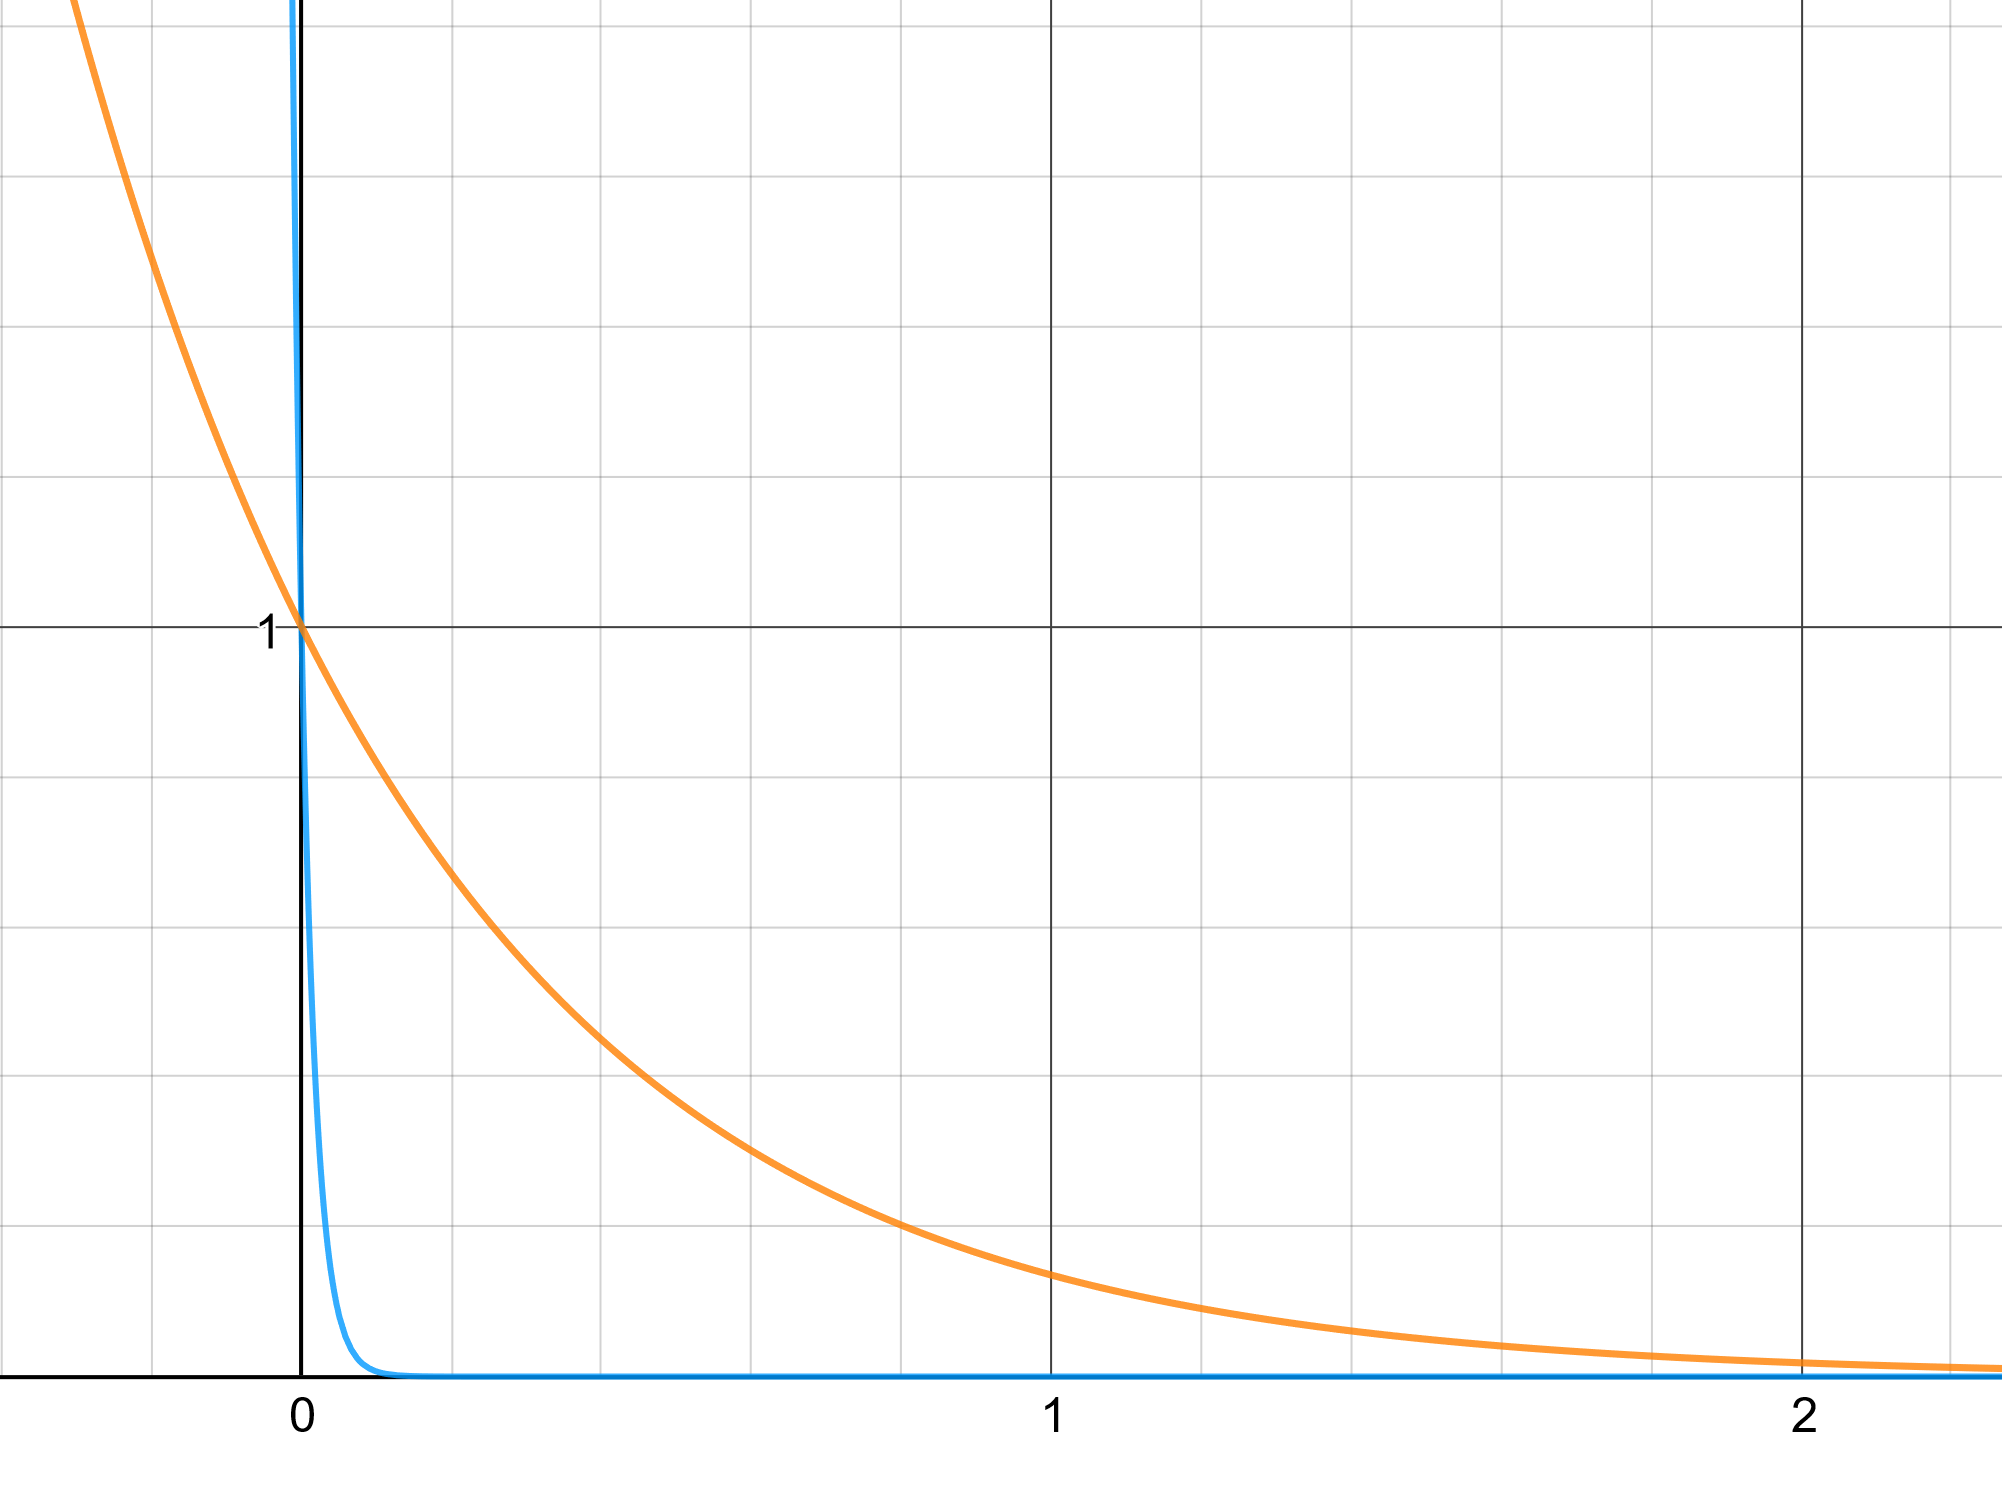
\includegraphics[width = 0.5\linewidth]{figures/e_expl_curve.png}
	\caption{Graph explaining the difference in acceptance rates (Generated at https://www.geogebra.org/graphing/g7kyzwce)}
	\end{figure}
	 
	%exp((posterior2-posterior1)/(abs(posteriorref)/50));
	
	
	\section{Optimisation to determine MAP}
The maximum a posteriori of the posteriori function was also determined to allow for further comparison of results.
All the values and constants except for the $\kappa$-values were kept the same as in the MCMC integration to allow the results to be compared on the same basis.  
	The optimisation to determine the maximum value of the posteriori function was initially done utilising the built in Matlab optimisation algorithm \texttt{femsearchmin.m}. 
	Since the built-in optimisation intends to minimise the function the probability was multiplied with -1 such that the minimum found is actually the maximum.
	After initial analysis the maximum was found at negative $\kappa$-values, as previously stated that is illogical and impractical.
	Further research on various adaptations of the built-in function lead to finding the \texttt{femsearchminbnd.m} adaptation by \citet{derrico:2021}. 
	This was used to limit the search area to only positive $\kappa$-values.
	Further the algorithm was set to only iterate a thousand times and stop if the points of the simplex are within 0.009.
	The start point for the algorithm was chosen to be the $\kappa$-values from the EURO code.
	
	
	
	
